\documentclass[11pt,a4paper,nolmodern]{moderncv}
\moderncvtheme[black]{classic} % color options 'blue' (default), 'orange', 'green', 'red', 'purple', 'grey' and 'black'               
%\usepackage[latin1]{inputenc}
\usepackage[utf8]{inputenc}
\usepackage{natbib}
\usepackage[scale=0.8]{geometry}
\usepackage[gen]{eurosym}
\usepackage{graphics}

\DeclareUnicodeCharacter{20AC}{\euro{}}

\firstname{Joseph}
\familyname{Scola}
\title{Maître de conférences -- CNU 28}              
\address{6 rue du Général Pershing}{78000, Versailles}    
\phone{06 03 69 32 40}                    
\email{joseph.scola@uvsq.fr}   
\extrainfo{41 ans}                   
%\homepage{www.uvsq.fr}

\newcommand{\etal}{\textit{et al.}}

\begin{document}
\maketitle

\pagestyle{empty}

\section{Physique des lacunes d'oxygène dans des films d'oxyde}
\cventry
	{}
	{Oxydes magnétiques, matériaux massifs, couches minces, hétérostructures, interfaces d'oxyde}{mesure de transport électrique, diffraction et réflectométrie des rayons X, grands instruments (champs forts, diffraction de neutron, rayonnement synchrotron), lithographie optique, mesure à haute température et cryogénie}{}{}{}
	
\section{Parcours scientifique}
%	{2015}
%	{Délégation CNRS (6 mois)}{}
%	{Groupe d'\'Etude de la Matière condensée (GEMaC), UMR 8635, Versailles}{}
%	{{\emph{Transition métal-isolant induite par sous-st\oe chiométrie d'oxygène dans des films
%de LaNiO$_3$ : structures atomique et électronique.
%}}}
%\cventry%
%	{2009}
%	{Délégation CNRS}{}
%	{UMR 8635, Groupe d'\'Etude de la Matière condensée, Versailles}{}
%	{{\emph{Couplage magnétique dans des hétérostructures tout-oxyde}} (6 mois)}
\cventry
	{depuis 2007}
	{Maître de conférences}{}
	{GEMaC - Université de Versailles St-Quentin (UVSQ)}{}
	{}%{\emph{Couplage magnétique dans des hétérostructures tout-oxyde}}
\cventry
	{2005-2007}
	{Post-doctorat}{}
	{CEA-Saclay, Service de Physique de l'\'Etat Condensé}{}
	{\emph{Fluctuations dans des jonctions tunnel magnétiques.}}
\cventry
	{2005}
	{Doctorat en milieux denses et matériaux}{}
	{Université de Caen}{}
	{\emph{\'Etude de la dynamique d'un réseau de vortex dans un supraconducteur par mesures de bruit.}}
\cventry
	{2002}
	{DEA d'électronique}{}
	{Université de Rouen}{}
	{Mémoire: \emph{Analyse en temps réel de transitoires multi-exponentiels.}}
\cventry
	{2002}
	{Diplôme d'ingénieur en Génie Mathématique}{}
	{Institut National des Sciences Appliquées}{}
	{Stage ingénieur: \emph{Décompositions en ondelettes de signaux musicaux.}}
	
\section{Contrats et financements}
	\cventry
	{2021-2025}
	{ANR SUPERNICKEL} {605 k€}{Resp. : A. Pautrat, Chercheur principal GEMaC. : J. Scola}{}
	{Synthesis and physical properties of new SUPERconducting NICKEL oxides (SUPERNICKEL).}
	
	\cventry
	{2013-2014}
	{Labex CHARM3AT valorisation} {55 k€}{Resp. J. Scola}{}
	{Optimisation de Colles Conductrices Haute Température à base de Nanoparticules d'Ag (ColCoNAg).}

	\cventry
	{2017-2018}
	{Mission Initiatives et Innovations Pédagogiques U. Paris-Saclay} {13 k€}{Resp. J. Scola}{}
	{Pédagogie par projet : accompagner les premiers pas à l'Université.}

\iffalse	
	\subsection{Partenariats}	
	\cventry
	{2009-2011}
	{Partenariat Hubert Curien Pessoa}{}{Resp. français: J. Scola, Resp. portugais: D. S. Schmool}{}
	{\emph{Spin dynamics and magneto-transport in all oxide magnetic multilayers.}}
\fi
	

\newpage 

\section{Fonctions d'intérêt collectif}
\cventry
	{depuis 2016}
	{Coordinateur de la cordée de la réussite de Physique}{}
	{UVSQ-Paris-Saclay}
	{Formation d'étudiant·e·s de licence de Physique à la médiation scientifique à destination d'élèves de collège}
	{}
\cventry
	{depuis 2016}
	{Membre du conseil scientifique du GDR MEETICC}{}
	{}
	{}
	{}
\cventry
	{2018}
	{Organisation d'une réunion thématique de GDR à Versailles}{}
	{Matériaux, Etats ElecTroniques, Interactions et Couplages non-Conventionnels (MEETICC)}
	{\emph{Techniques avancées: focus sur les oxydes, supraconducteurs 2D et dichalcogénures}}
	{}
\cventry
	{2018}
	{Comité de sélection du poste de maître de conférences n$^\circ$ 0021 (CNU 28, 31, 33)}{}
	{Département de physique, CentraleSupélec, SPMS}
	{\emph{Physique, état solide, matériaux, simulation, ab-initio}}{}
%%%%%%%%%%%%%%%%%%%%%%%%%%%%%%%%%%%%%%%%%%%%%%%%
\iffalse
\cventry
	{2014}
	{Co-organisation d'un mini-colloque de la Condensed Matter in Paris (CMD25-JMC14)}{}
	{divisions Matière Condensée des Sociétés européenne et française de Physique}
	{\emph{Strongly correlated systems I: Recent advances on metal-insulator transitions of correlated matter}}
	{}
\cventry
	{2011}
	{Comité de sélection du poste de maître de conférences n$^\circ$ 0108 (CNU 28)}{}
	{Institut Galilée, Université Paris 13}
	{\emph{Physique des matériaux fonctionnels et couplage}}{}
\cventry
	{2010}
	{Comité de sélection du poste de maître de conférences n$^\circ$ 0791 (CNU 28)}{}
	{Université de Versailles St-Quentin}
	{\emph{Auto-organisation dans les solides moléculaires photo-commutables}}{}
\cventry
	{2010-2015}
	{Président de jury}
	{Semestre 2 de la première année de Licence, parcours Physique-Chimie}
	{}
	{}{}	
\fi
%%%%%%%%%%%%%%%%%%%%%%%%%%%%%%%%%%%%%%%%%%%%%%%%
%\cventry
%	{depuis 2005}
%	{Rapporteur pour Physical Review B}{}{}{}{}
%\cventry
%	{depuis 2009}
%	{Responsable d'un instrument de service commun (magnétomètre à SQUID)}{}
%	{Groupe d'\'Etude de la Matière condensée, Versailles}{}{}
%\cventry
%	{2002-2005}
%	{Représentant des étudiants au conseil du laboratoire durant la thèse}{}{}{}{}

%\section{Intérêts extra-scientifiques}
%\cvitem{Sport}	{Karaté, ceinture noire troisième dan}{}{}{}{}
%\cvitem{Musique}{Diplôme d'\'Etude Musicale du CNR de Caen (Jazz)}{}{}{}{}
%\cvitem{}		{Diplômes de fin d'\'Etude du CNR de Caen (piano et solfège)}{}{}{}{}

\newpage
\input{resume.tex}

\newpage
\section{Activités d'enseignement}
\cventry
	{Licence 1}
	{Méthodologie pour la physique (Responsabilité de module, CM, TD, TP)}
	{licence math-physique-chimie}
	{(depuis 2018)}{}{}
\cventry
	{}
	{Mécanique générale (Responsabilité de module, CM, TD, TP)}
	{licence math-physique-chimie-informatique}
	{(2010-2020)}{}{}
\cventry
	{}
	{Optique géométrique et électrocinétique (TD, TP)}
	{licence math-physique-chimie-informatique}
	{(2007-2020)}{}{}	
\cventry
	{}
	{Physique pour la PACES (TD)}
	{Première année commune aux études de santé}
	{(2007-2017)}{}{}
\cventry
	{}
	{\'Electronique analogique et numérique (TD)}
	{licence math-physique-chimie-informatique}
	{(2007-2009)}{}{}

\cventry
	{Master 1}
	{Calculs scientifiques (Responsabilité de module, CM, TD, TP)}
	{master Physique, mécanique et science pour l'ingénieur}
	{(2010-2015)}{}{}
	
\cventry%
	{}	%
	{Mesures magnétiques (TP)}
	{master Physique et science pour l'ingénieur}
	{(2010-2012)}{}{}	

\cventry
	{Master 2}
	{Physique et Chimie de la Matière (Responsabilité de module, cours, TD)}
	{master Polymères et Biomatériaux (U. Paris-Saclay)}
	{(depuis 2015)}
	{}{}

\cventry
	{}
	{Physique des semiconducteurs, hétérostructures (TD)}
	{master Matériaux, Technologies et Composants: Photovoltaïque - Voiture Electrique}
	{(2011-2018)}
	{}{}

\iffalse
\cventry
	{}
	{Expériences récentes en Physique quantique (TD)}
	{master Nanosciences (U. Paris-Saclay)}
	{(2013)}
	{}{}
\fi

\cventry
	{}
	{Tuteur de stage}
	{master Métiers de l'Enseignement, de l'\'Education et de la Formation}
	{(depuis 2018)}
	{}{}

\cventry
	{Formation continue}
	{Physique générale (CM, TD)}
	{Diplôme d'accès aux études universitaires, Sciences}
	{(2016-2018)}{}{}


\section{Encadrement d'étudiants}
\cventry
	{Thèse}
	{Co-encadrant}
	{Nanoparticules d'argent pour l'électronique}
	{Yana Veniaminova, 2010-2013}
	{Co-tutelle GEMaC (CNRS-UMR8635) - ILV (CNRS-UMR8180)}{}

\cventry
	{Stages M2}
	{Encadrant}
	{Matériaux pour la récupération d’énergie : propriétés mécaniques de nanofils de ZnO}
	{Idris Aboubakari, 5 mois}	
	{}{}
	
\cventry
	{}
	{Encadrant}
	{Interface Al/ZnO : émergence de propriétés à l'échelle nanométrique}
	{Cheikh Samb, 2019, 4 mois}	
	{}{}
	
\cventry
	{}
	{Encadrant}
	{Mécanisme de conduction dans le métal à fortes corrélations électroniques LaNiO$_3$}
	{Abdelnour Benamar, 2016, 5 mois}	
	{}{}

\cventry
	{}
	{Encadrant}
	{Mesure de résistance à 1000 K}
	{Maya Taoui, 2014, 5 mois}	
	{}{}

\cventry
	{}
	{Encadrant}
	{Nanomatériaux pour l'interconnexion de cellules photovoltaïques à concentration}
	{Nour El Houda Kriden, 2014, 5 mois}
	{}{}
	
\cventry
	{Projet de fin d'étude INSA}
	{Co-encadrant}
	{Simulation numérique d'un antiferromagnétique canté par un modèle macro-spin}
	{Maxime Vallée, 2010, 6 mois}
	{Co-tutelle GEMac - Laboratoire de mathématique de l'INSA de Rouen}{}
	
\cventry
	{Stage M1}
	{Encadrant}
	{Influence des lacunes d'oxygène sur la structure électronique du métal corrélé
	LaNiO$_{3-\delta}$}
	{Mohammed Jamali, 2017, 4 mois}{}{}
	
\cventry
	{Stages L3}
	{Encadrement de 10 binômes en stage d'un mois depuis 2008}
	{}
	{}	
	{}{}

\iffalse
\cventry
	{Stages L3}
	{}
	{"Oxytronique : de l'expérience à la médiation scientifique"}
	{2015, 1 mois}	
	{}{}

\cventry
	{}
	{}
	{"Propriétés magnétiques de nanoparticules magnétiques fonctionnalisées"}
	{2013, 1 mois}	
	{}{}

\cventry
	{}
	{}
	{"Résolution numérique de l'équation de la chaleur"}
	{2011, 1 mois}	
	{}{}
	
\cventry
	{}
	{}
	{"Protocole d'utilisation du Physical Properties Measurement System"}
	{2010, 1 mois}	
	{}{}

\cventry
	{}
	{}
	{"Protocole d'utilisation d'un bâti de pulvérisation cathodique"}
	{2009, 1 mois}	
	{}{}	

\cventry
	{}
	{}
	{"Magnétométrie SQUID"}
	{2009, 1 mois}
	{}{}	

\cventry
	{}
	{}
	{"Conception et réalisation d'amplificateurs analogiques faible bruit"}
	{2008, 1 mois}
	{}{}		
	
%\iffalse	
\section{Contributions au département de physique}
\cventry
	{2012}
	{Médiation scientifique}{}
	{UVSQ}
	{Organisation d'une conférence sur \emph{Le boson de Higgs} par G. Cohen-Tannoudji}
	{}{}{}

\cventry
	{2010-2015}
	{Président de jury}
	{Semestre 2 de la première année de Licence, parcours Physique-Chimie}
	{}
	{}{}	
\fi

\newpage
\section{Activités de recherche}

Mon activité principale concerne la physique des lacunes d'oxygène dans des films d'oxydes :
caractériser les défauts lacunaires, comprendre leur influence sur les propriétés macroscopiques et les utiliser pour fonctionnaliser les matériaux.
J'ai mené ma recherche dans le Groupe d'\'Etude de la Matière condensée (GEMaC, UMR 8635) dans l'équipe oxydes magnétiques fonctionnels jusqu'à 2018.
Depuis 2019, cette activité se poursuit au sein de l'équipe Nanostructures Semiconductrices et Propriétés dirigée par V. Sallet; ce changement m'a permis de bénéficier d'un cadre thématique et d'un soutien technique plus appropriés.
%J'y prolonge mon activité de recherche concernant les interfaces d'oxyde sur les systèmes MgZnO/ZnO et Al/ZnO, dans la continuité de mon étude précédente de l'interface Al/LaNiO$_3$. Il s'agit d'investigations conjointes des morphologies d'interface (sondée par diffraction et réflectivité de rayons X) et des propriétés électriques (microstructuration de croix de Hall et mesure de transport).

J'ai pris en charge les expériences d'indentation par microscope à force atomique et de réflectométrie de rayons X (alignement du chemin optique, rédaction du protocole expérimental, établissement d'une base de données de référence et rédaction d'un programme original de simulation des données jusqu'à 4 couches rugueuses).
Je participe également aux expériences de mesure de transport (PPMS 9 T) et de diffraction de rayons X pour le laboratoire (développement de logiciels de simulation de l'espace réciproque et de visualisation de cartographie de l'espace réciproque).

%Je mentionne également une activité moins récente mais en lien avec le projet que je présente.
%Il s'agit de l'étude de la microstructure de colles conductrices à base de nanoparticules d'argent pour des application à haute température ; cette activité a été financée sur projet (Labex CHAR3MAT) et impliquait un ingénieur contractuel et deux stages de M2.

%Dans la continuité des mes travaux antérieurs au GEMaC, j'ai poursuivi une activité de recherche subsidiaire portant sur la mesure de propriétés magnétiques.
%Le projet le plus fructueux a concerné des nanoparticules de ferrites greffées sur des matériaux microporeux destinés à des applications médicales (synthétisées à l'Institut Lavoisier de Versailles, UMR 8180 du CNRS).
%Cette action de recherche a été financée par la région Ile-de-France (c'Nano).

\bigskip
\textbf{\textsf{Analyse ionique de films de nickelates supraconductrices}}

La découverte de supraconductivité en 2018 dans des films de Nd0,8Sr0,2NiO2 [D. Li et al., Nature 572, 624–627 (2019)] a drainé une attention considérable : recherchée depuis trois décennie, la supraconductivité dans des composés analogues aux cuprates suscite l’espoir d’offrir une nouvelle perspective sur la supraconductivité à haute température critique et d’éclairer enfin la Physique de ce phénomène. La synthèse de nickelates supraconductrices n’a été à ce jour réalisée que par un petit nombre de groupes dans le monde [S. Zeng et al, Phys. Rev. Lett. 125, 147003 (2020), Y. Zaing et al, Chin. Phys.Lett. 38, 047401 (2021)]. Le consortium du projet ANR SUPERNICKEL (2022-2025) a été constitué pour atteindre cet objectif en France.
Les nickelates supraconductrices actuellement produites sont élaborées par croissance de la phase perovskite suivie d’une réduction topotactique sous atmosphère de CaH2. L’analyse par spectroscopie d’ions secondaires (SIMS), dont j’ai la charge dans le projet, répond à la nécessité de contrôler finement les compositions, en particulier celles des éléments légers. L’enjeu est en effet de maîtriser l’évolution de la stœchiométrie en oxygène au cours de la réduction et de déterminer la quantité d’hydrogène introduite en concomitance. La présence d’hydrogène a été détectée en 2023 par SIMS [Ding, X., Tam, C.C., Sui, X. et al. Critical role of hydrogen for superconductivity in nickelates. Nature 615, 50–55 (2023)] et la question se pose maintenant d’en quantifier la concentration afin d’élucider sa contribution à la supraconductivité.
L’analyse quantitative d’une intensité ionique est rendue difficile du fait qu’elle dépend de facteurs très sensibles à l’environnement chimique et qui doivent être estimés avec précaution. Nos efforts à Versailles ont donc porté sur l'analyse d'échantillons de références, élaborés par le CRISMAT de Caen et le GREMAN de Tours, pour déterminer les facteurs expérimentaux pour l’analyse quantitative de nickelates supraconductrices. Il a ainsi été possible de déterminer l’influence de l’environnement chimique avec le taux d’ionisation, le rendement de pulvérisation ionique et les facteurs de collecte de l’appareil. De plus, l’optimisation et la modélisation du mécanisme de pulvérisation a permis d’atteindre une résolution en profondeur inférieure à 10 nm (voir figure ci-dessous), permettant ainsi l’analyse de films ultra-minces. Sur cette base, nos analyses ont déjà pu mettre en évidence les effets de la réduction sous CaH2 sur les films non supraconducteurs du consortium. Une partie de ces travaux ont été réalisés dans le cadre du stage M2 de M. Julien Garcia.


Les figures suivantes montrent, à gauche, les intensités ioniques de $^{88}$Sr et $^{138}$Ba le long du gradient latéral de composition d’une couche de Ba$_x$Sr$_(1-x)$TiO$_3$ et à droite le profil d’intensité de $^{139}$La au franchissement de l’interface La$_{0,9}$Sr$_{1,1}$NiO$_4$/SrTiO$_3$ et sa modélisation (en pointillés rouges) dont le paramètre ajustable indique un élargissement instrumental de 5 $\pm$ 2 nm.
\par
\begin{center}
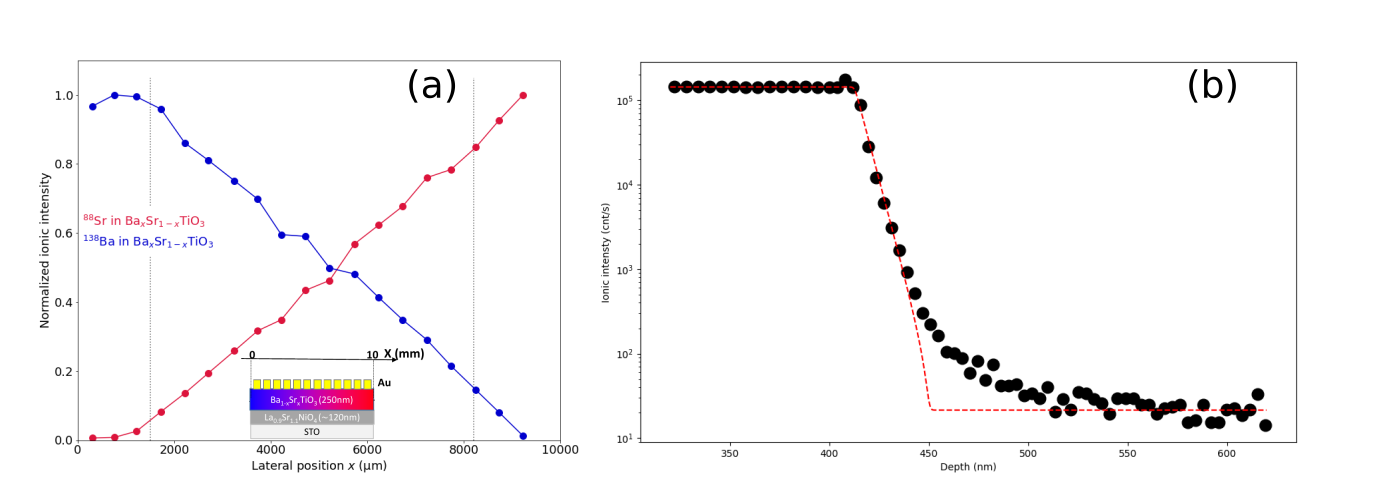
\includegraphics[width=0.85\textwidth]{./figures/SUPERNICKEL.png}
\end{center}







	\bigskip
	\textbf{\textsf{Physique des lacunes d'oxygène dans des films d'oxydes de structure perovskite}}

La structure électronique des nickelates de terres rares (structure perovskite) résulte de la compétition entre plusieurs interactions proches en énergie : des transitions structurales et magnétiques accompagnent la transition métal-isolant qui s'y tient.
Celle-ci se produit en température, mais peut-être également être induite dans des films minces par substitution chimique, pression biaxiale, confinement, ou effet d'interface. Ces procédés ont été appliqués avec succès au composé LaNiO$_3$ pour induire l'état isolant qui n'a jamais été observé dans le matériau natif. Le contrôle par un champ externe de la transition métal-isolant dans les nickelates et particulièrement dans LaNiO$_3$ constitue un enjeu expérimental central dans la thématique des nickelates.

Il est établi depuis près de vingt ans que l'introduction de lacunes d'oxygène supprime la conduction électrique dans LaNiO$_3$. 
L'approche que je mène consiste à exploiter la st\oe chiométrie en oxygène. Ma problématique de recherche consiste ainsi à (1) mesurer la concentration de lacunes d'oxygène crées dans un film par un procédé donné, (2) en décrire la distribution spatiale, et en l'occurrence la mise en ordre des lacunes pour une concentration donnée et (3) développer des procédés de contrôle réversible de la concentration de lacunes dans un film.

\textbf{Mesure de la concentration de lacunes d'oxygène.}
L'étude de la concentration de lacunes d'oxygène s'appuie sur le spectromètre de masse d'ion secondaire (SIMS 7f) dont dispose le GEMaC. Le principe de la technique consiste à comparer la concentration d'oxygène du film mesuré avec un film de référence. L'application de cette technique pour la mesure de la st\oe chiométrie en oxygène de films d'oxyde est une innovation expérimentale permise par la grande résolution de l'équipement nouvellement acquis par le laboratoire. Une résolution de 5 \%  sur la variation de concentration a été obtenue et la résolution spatiale est de 10 nm en profondeur (pour une surface sondée de 10 $\mu$m x 10 $\mu$m).
En outre, l'avantage de l'analyse par SIMS est qu'elle permet de contrôler simultanément le rapport cationique.

Cette expérience a permis de déterminer le rendement de désoxygénation et de réoxygénation pour différents  protocoles de recuit sous vide ou sous oxygène (en utilisant un marqueur ${}^{18}$O) appliqués à plusieurs films d'oxydes de structure perovskite.
Le résultat marquant de cette campagne d'expérience a été la mise en évidence de l'influence de l'orientation cristallographique sur le rendement des échanges d'oxygène des surfaces.
Par ailleurs, les propriétés de filtrage d'oxygène d'une sur-couche superficielle de LaAlO$_3$ ont été vérifiées et l'impact sur le rendement des échanges d'oxygène a pu être mesuré quantitativement.
Enfin, l'étude a montré que la concentration des lacunes est uniforme dans l'épaisseur du film et il a été possible de distinguer la mobilité de l'oxygène dans les couches de celle dans le substrat de SrTiO$_3$.

\textbf{Morphologie des films sous-st\oe chiométriques.}
Une fois la concentration de lacunes d'oxygène estimée, leur distribution dans le volume des films a fait l'objet d'une étude approfondie par diffraction de rayons X au GEMaC et par microscope électronique à transmission (TEM) et spectroscopie de perte d'énergie des électrons (EELS), en collaboration avec le SPMS (CentraleSupélec).
Les films st\oe chiométriques s'avèrent exempts de défauts à proximité de l'interface, et au-delà présentent quelques défauts plans de type parois de macle.
La présence de lacunes d'oxygène  conduit à l'apparition de deux nouvelles phases, à savoir une phase Ruddlesden-Popper et une phase de type Brown-Millerite.
Dans cette dernière, il a été mis en évidence l'absence de symétrie d'inversion par diffraction par faisceau convergent.
Par ailleurs, l'expérience de microscopie, combinée à une analyse spectroscopique des pertes d'énergie des électrons a permis dans certains cas de mettre en évidence des distributions non-uniformes de la valence du nickel, et donc indirectement de la concentration de lacunes d'oxygène.

Cette étude a été complétée par une expérience de diffraction en incidence rasante sur la ligne SixS du synchrotron SOLEIL.
Les résultats préliminaires confirment la présence de défauts planaires dans les films st\oe chiométriques et informent sur les différents variants en présence.



\textbf{Pilotage des lacunes d'oxygène : renforcement de l'effet Schottky par transport de masse réversible, à température ambiante.}
Le dépôt d'une couche d'un métal réducteur sur un oxyde entraîne la création de lacunes d'oxygène dans l'oxyde à proximité de l'interface et l'oxydation du métal sur quelques nanomètres.
Ce procédé a récemment prouvé son utilité pour créer un système électronique bidimensionnel sur une surface de SrTiO$_3$. J'ai mené une étude s'appuyant sur ce principe et portant sur des contacts Al/LaNiO$_3$. La résistance perpendiculaire, c'est-à-dire à travers la couche d'aluminium puis celle de LaNiO$_3$, présente un comportement non-ohmique.

La morphologie de l'interface Al/LaNiO$_3$ a été étudiée conjointement par microscopie électronique à transmission (TEM), analyse dispersive en énergie (EDS) et réflectométrie de rayons X sur la ligne SixS du synchrotron SOLEIL (XRR) pour des orientations de surface (001) et (111).
Ces expériences ont confirmé la diffusion d'atomes d'oxygène, mais également de l'interdiffusion de nickel et d'aluminium, sur des distances de quelques nanomètre.
Il en résulte la formation spontanée de composés intermédiaires à l'interface Al/LaNiO$_3$.
Ces déplacements atomiques se produisent en phase solide, en-dessous de 200 $^\circ$C, et se trouvent favorisés par la présence et la mise en ordre de défauts lacunaires dans l'oxyde.

Les figures ci-après montrent les images chimiques obtenues par EELS (à gauche), les profils d'interface reconstitués (au milieu); la réflectivité de rayonnement synchrotron peut être modélisée par une morphologie très proche de celle obtenue localement par microscopie, ce qui confirme la formation de composés intermédiaires sur l'ensemble de l'interface (à droite).
\par
\includegraphics[width=0.33\textwidth]{./figures/TEM_HR_EDS.eps}
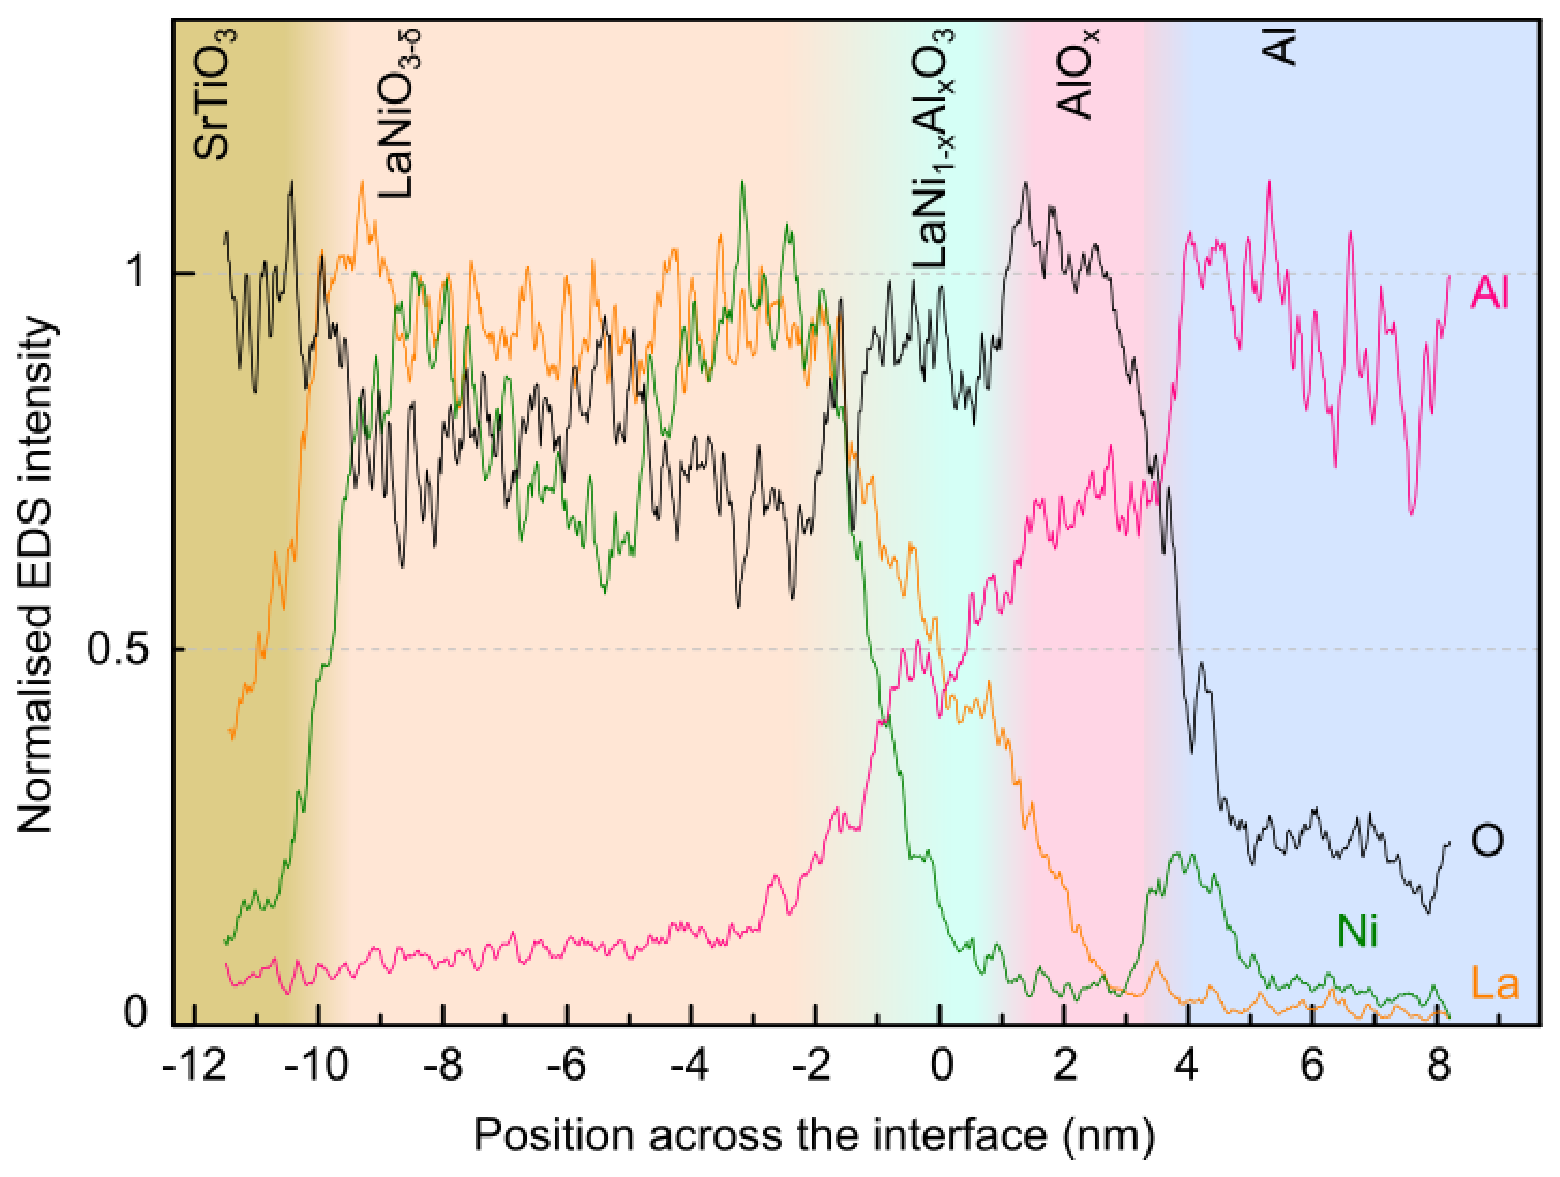
\includegraphics[width=0.33\textwidth]{./figures/TEM_EDS_profiles_inverted.eps}
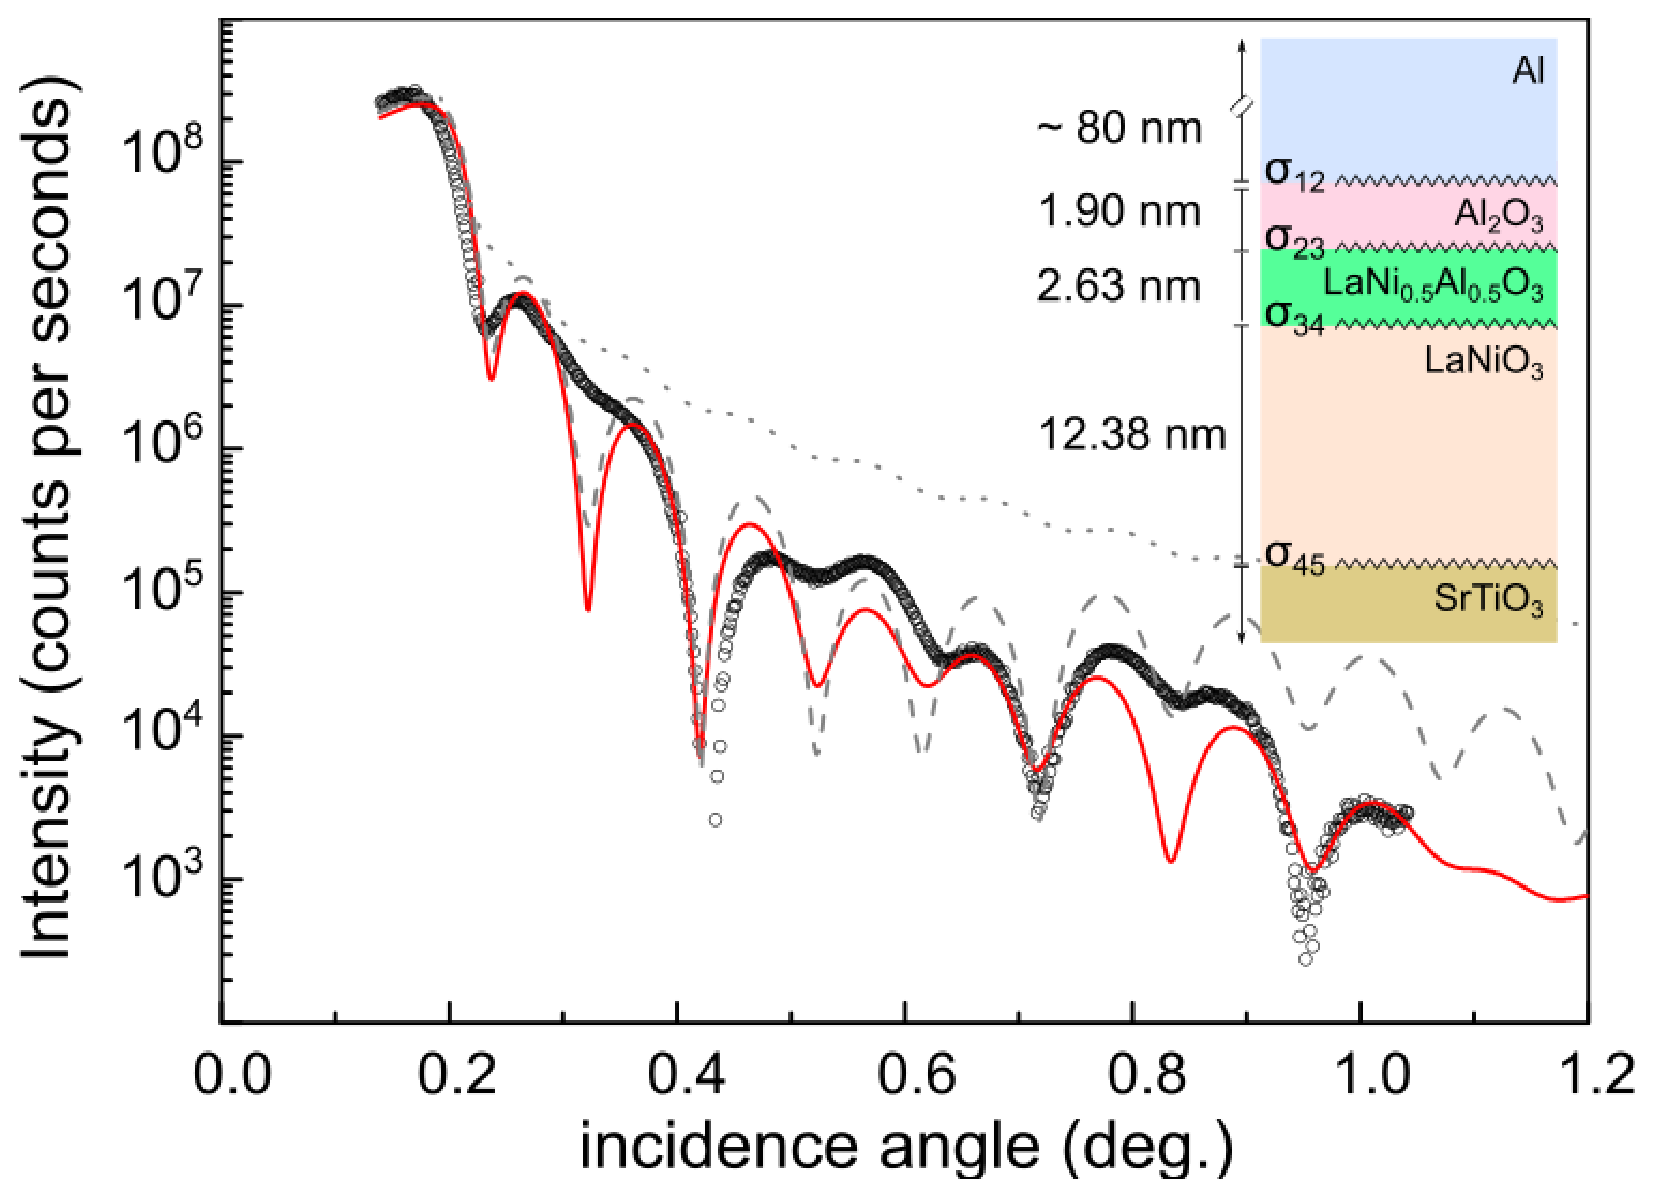
\includegraphics[width=0.33\textwidth]{./figures/XRR_OFFState3.eps}

La caractéristique courant-tension I(V) de cette structure correspond à celle d'une diode, ce qui est remarquable pour l'empilement de deux métaux.
Ce comportement est la conséquence d'une réaction d'oxydo-réduction se produisant en phase solide à l'interface Al/LaNiO$_3$.
Suivant le sens de polarisation en tension ($\pm$ 5 V), la résistance varie d'un facteur jusqu'à 1000 à température ambiante et 10000 à 5 K.
En polarisation directe, la résistance du contact ainsi que sa dépendance en température correspondent à celles d'un film de LaNiO$_3$ (la résistance de l'aluminium est négligeable). 
Le contact n'est pas de type Schottky du fait que l'augmentation de la tension inverse réduit la résistance du contact.
La dépendance du courant $I$ en $V^{1/2}$ et de $\ln I$ en fonction de $T^{2}$ indiquent qu'il s'agit plutôt d'une émission thermionique à travers les points faibles (les surfaces actives sont de l'ordre de 50$\times$50 nm$^{2}$) de la barrière de potentiel (de l'ordre de 100 meV) spontanément formée à l'interface (voir la figure ci-dessous).
\par 

\includegraphics[width=0.33\textwidth]{./figures/cadre_blanc.eps}
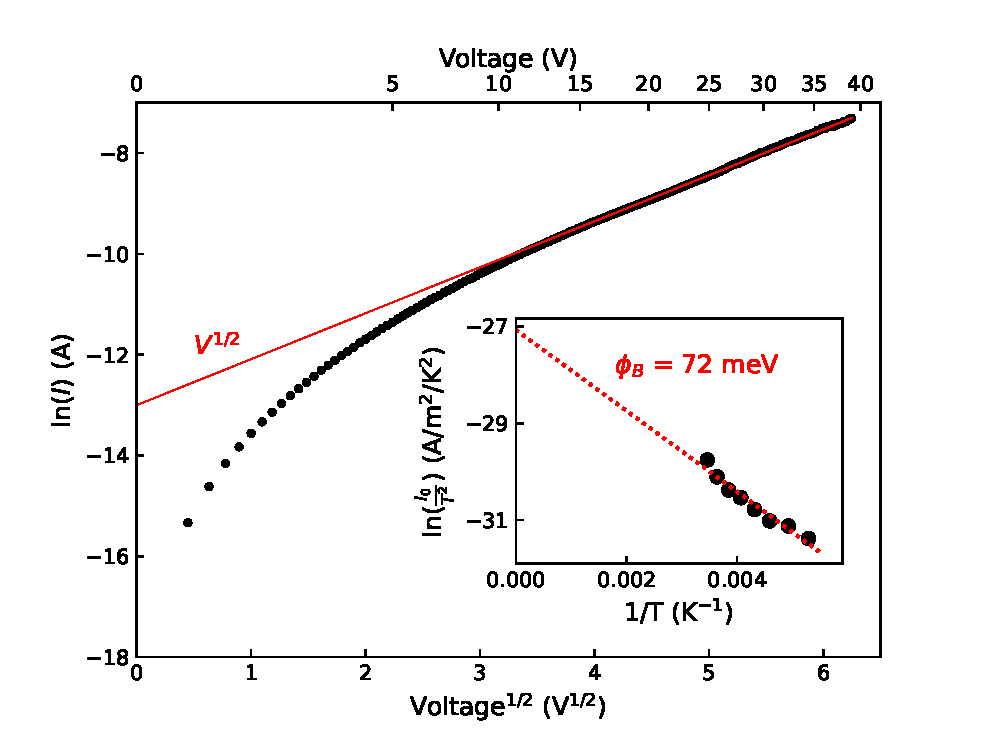
\includegraphics[width=0.33\textwidth]{./figures/G434_TE_IV.eps}

\includegraphics[width=0.33\textwidth]{./figures/cadre_blanc.eps}

La polarisation directe a pour effet d'injecter dans la région réduite (1) des trous libres, majoritaires dans la région non réduite de LaNiO$_3$, et (2) des ions O$^{2-}$ accumulés dans la l'oxyde d'aluminium.
La réaction d'oxydo-réduction se trouve ainsi inversée et les matériaux retrouvent leurs propriétés métalliques natives.


%L'ensemble de ces travaux fait est présenté dans un manuscrit et en cours de révision par ACS Applied Materials and Interfaces.

	\bigskip
	\textbf{\textsf{\'Etude des propriétés mécaniques de nanofils de ZnO par indentation et cartographie microscope à force atomique}}

Ce travail s'inscrit dans le cadre de la prospection de nouveaux matériaux pour la production et la récupération d'énergie. Les sources de déformations ou de vibrations mécaniques sont omniprésentes et disponibles en permanence. Par exemple, la récupération d'une fraction de l'énergie biomécanique générée par le corps humain (0.9 W pour la circulation sanguine jusqu'à 60 W des impacts se produisant lors de la marche à pied) pourrait alimenter des implants médicaux de basse consommation comme un pacemaker.
%
Les nanofils offrent de nombreux avantages pour la conversion électromécanique d'énergie. La taille réduite qui les caractérise est bien sûr tout à fait adaptée à une intégration dans des systèmes compacts. De plus, leur rapport d’aspect exalte les propriétés piezoélectriques, ce qui améliore l’efficacité de la récupération d’énergie.

Deux verrous doivent encore être levés pour tirer partie de tous ces avantages : la relative faiblesse du couplage électromécanique et le manque d'information concernant la robustesse et les mécanismes de défaillance des dispositifs, notamment des nanofils. A l'heure actuelle, un des objectifs à atteindre pour une production industrielle de tels systèmes d'alimentation autonomes est la fabrication de dispositifs autonomes. L'autonomie ne faisant de sens que pour des durées de vie longues, la fiabilité constitue un critère incontournable. Cela confère une importance particulière à la robustesse mécanique des nanofils.

Cette étude était l'objet du stage M2 de M. Idris Aboubakari qui a réalisé les mesures des propriétés mécaniques d’une assemblée de nanofils enduits de résine polymère.
Ce travail a inclut la mise en \oe uvre les dépôts de polymère, le polissage des surface et la cartographie des propriétés mécaniques au moyen d’un microscope à force atomique. 
Une procédure de calibation a été développée pour extraire des mesures de nano-indentation les modules d'Young locaux.

\begin{center}
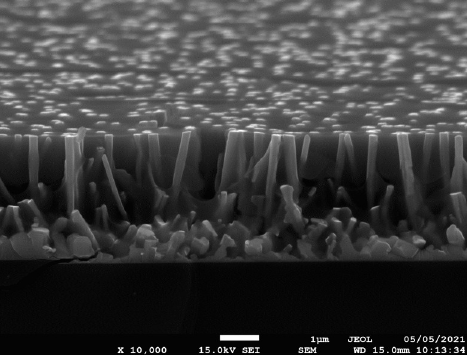
\includegraphics[height = 0.19\textwidth]{./figures/Polished_ZnONW_at_SOG_MEB.png}
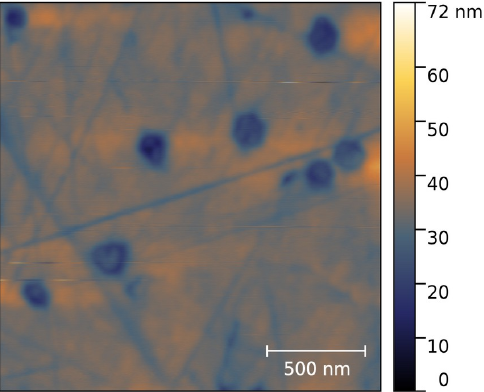
\includegraphics[height = 0.19\textwidth]{./figures/Polished_ZnONW_at_SOG_AFM.png}
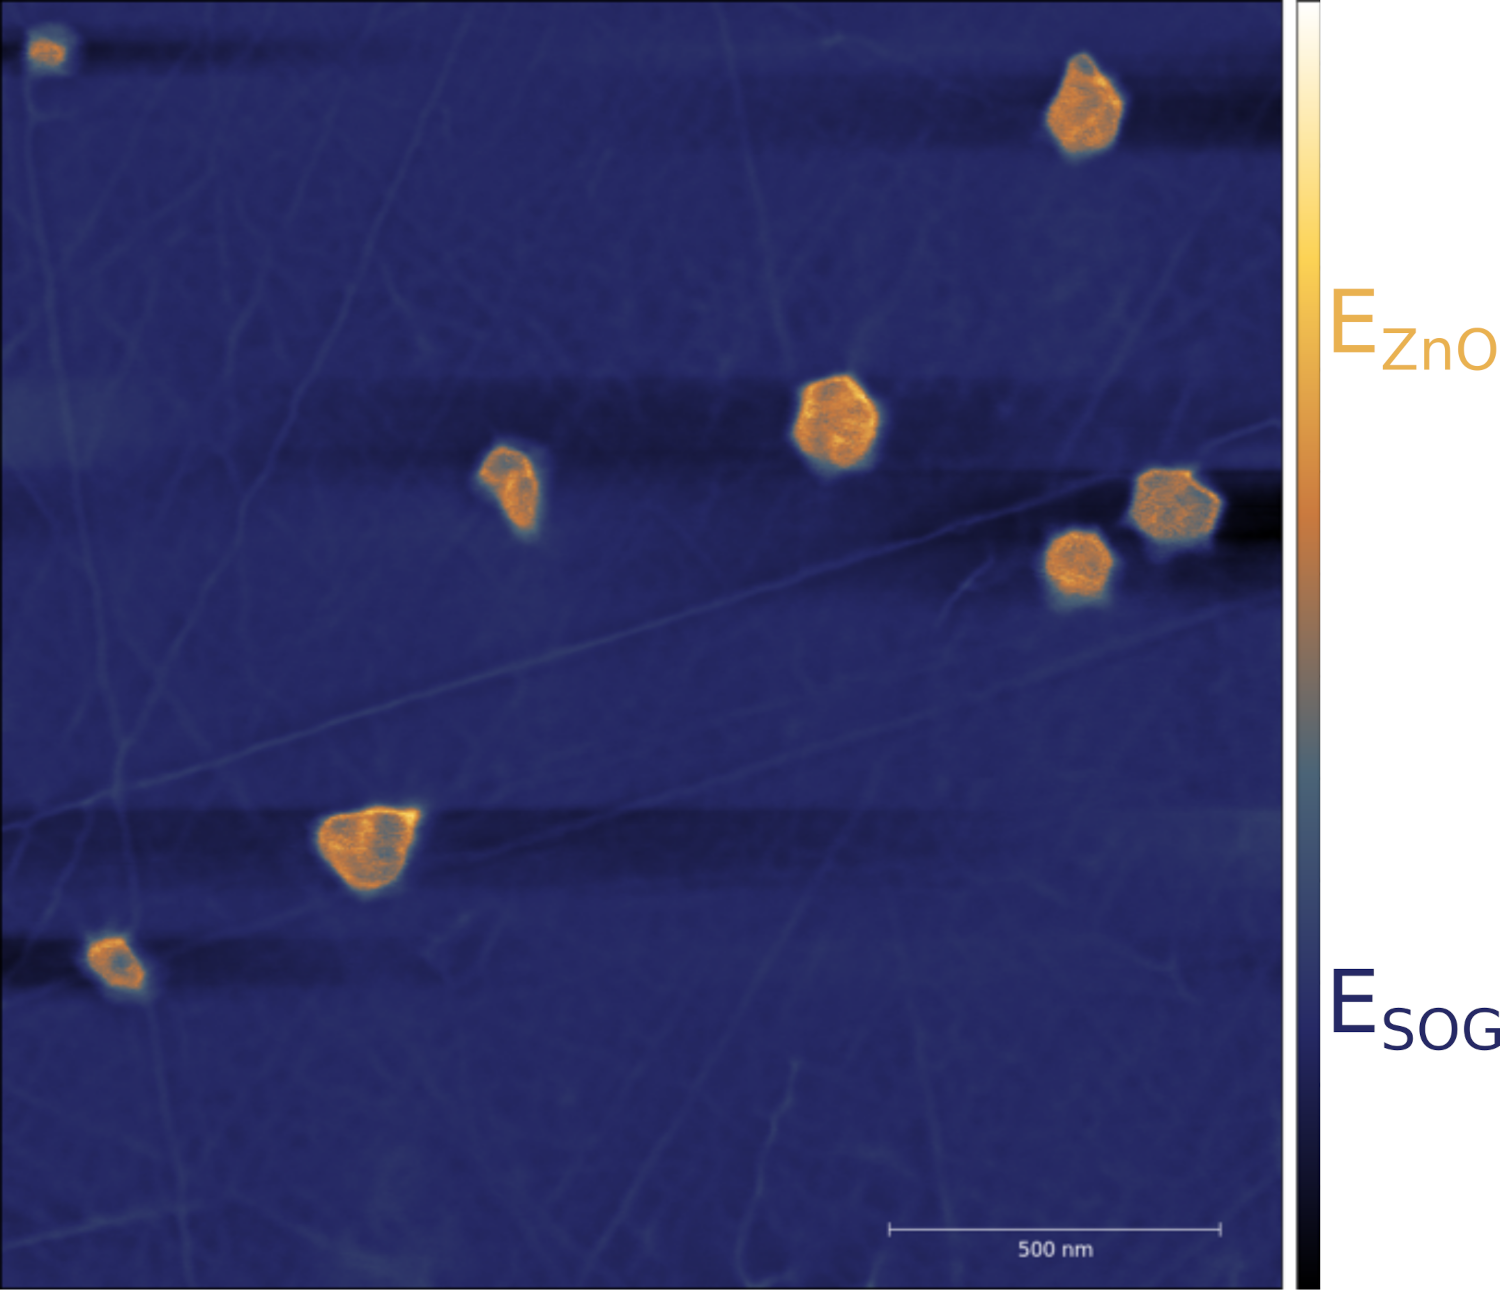
\includegraphics[height = 0.19\textwidth]{./figures/Polished_ZnONW_at_SOG_QNM.png}
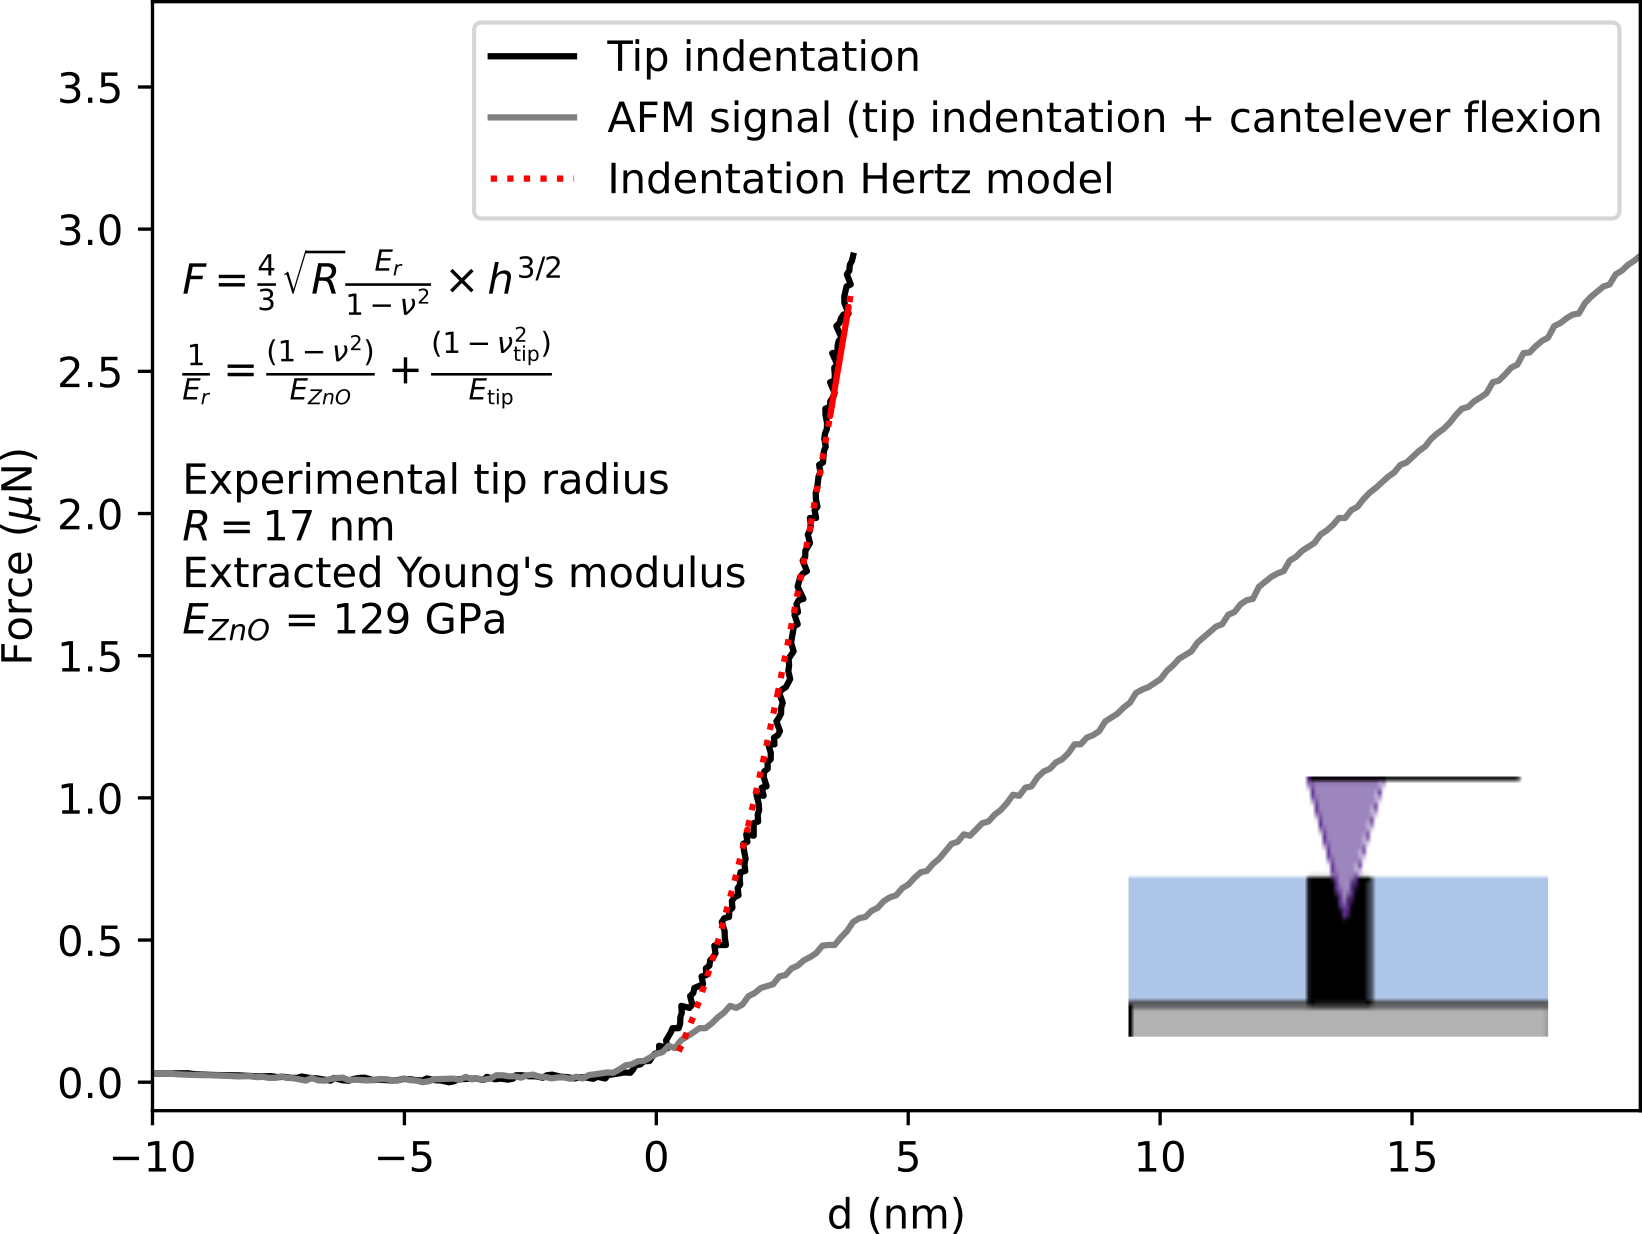
\includegraphics[height = 0.19\textwidth]{./figures/Polished_ZnONW_at_SOG_Indent.png}
\end{center}
Image de gauche : vue de microscopie électronique à balayage d'une coupe transverse d'un composite de nanofils de ZnO enduits d'une matrice rigide de spin-on-glass, après polissage.
Image centre-gauche : image topographique de la surface du même composite par microscope à force atomique.
Image centre-droit : cartographie de l'élasticité locale sondée sur la même zone.
Image de droite : courbe d'indentation avant et après extraction de la déflexion du cantilever; la rayon et la déformation de la pointe sont déterminés par indentation d'étalons.


	\bigskip
	\textbf{\textsf{Développement instrumental et logiciel pour la diffraction et la réflectométrie de rayons X au GEMaC}}
	
J'ai consacré ma première année (et le confinement) dans l'équipe NSP à développer des outils d'analyse et de simulation pour la diffraction et la réflectivité de rayons X.
\'Ecrit en python, ces outils incluent la représentation dans l'espace direct de la maille élémentaire, la représentation en 3D des réseaux direct et réciproque ainsi qu'une coupe de l'espace réciproque pour une orientation arbitraire.
Les figures ci-dessous illustrent ces fonctionnalités pour le composé Ruddlesden-Popper Sr$_3$Ti$_2$O$_4$ : à gauche, une représentation 3D de la position des atomes et à droite, un coupe de l'espace réciproque pour les directions orthogonales à (110) (les taches de Bragg sont indexées et leurs intensités théoriques sont représentées par la taille du point).
\par
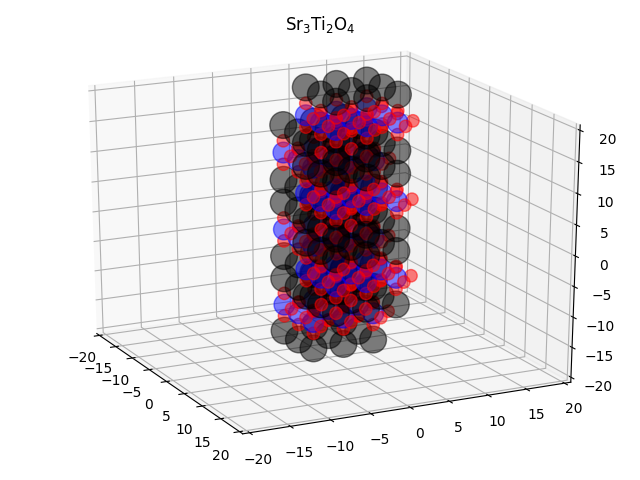
\includegraphics[width=0.5\textwidth]{./figures/RP1_Cell_Drawer.png}
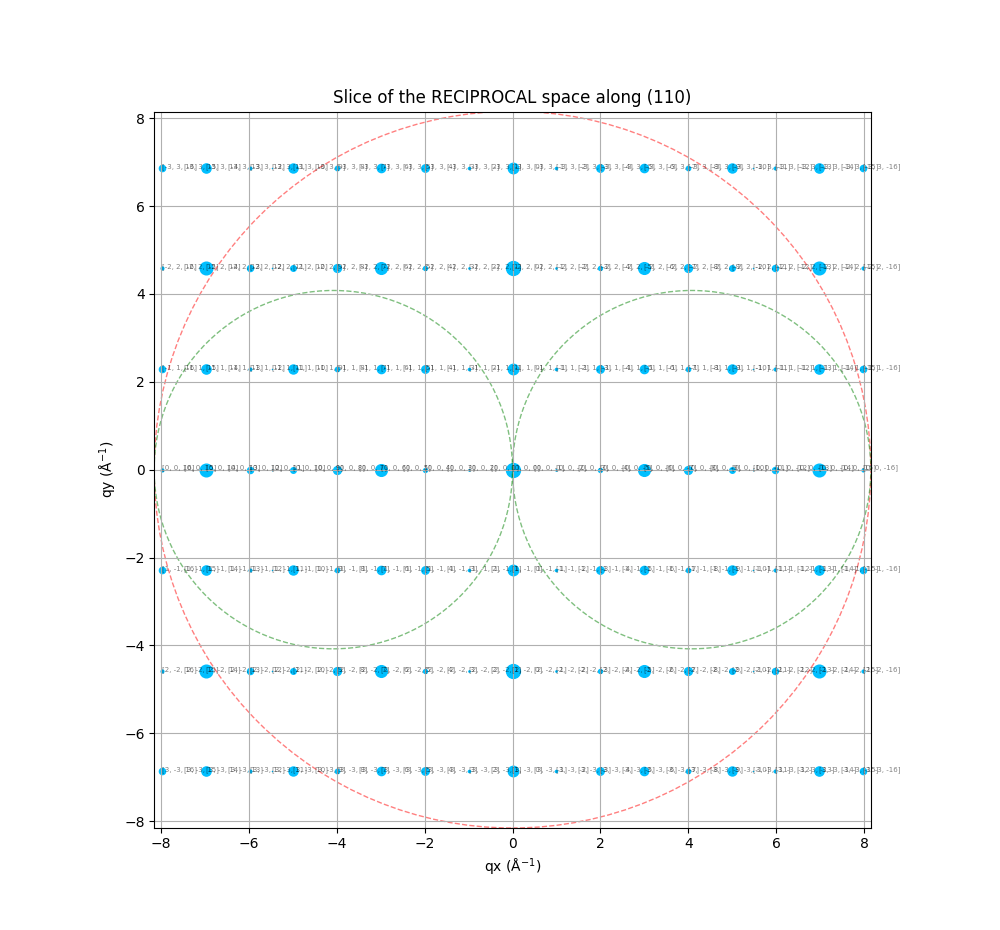
\includegraphics[width=0.5\textwidth]{./figures/RP1_RSSlice.png}

Mon activité a été motivée à la fois par les besoins du GEMaC de disposer d'une expérience de caractérisation de routine par réflectivité de rayons X et par les efforts requis pour l'analyse d'une expérience de réflectivité de rayonnement synchrotron que j'avais menée à SOLEIL en 2018.
D'un point de vue expérimental, il s'agissait de rattraper une perte de savoir-faire en réactivant un montage dont le fonctionnement avait été interrompu (alignement, réglage, établissement d'un protocole utilisateur et mesures de références).
Pour analyser les résultats, il a été nécessaire de développer un programme de simulation de l'intensité réfléchie : le programme calcul les indices optiques à partir des coefficients de diffusion atomique et simule jusqu'à 4 couches en tenant compte des rugosités d'interface.
La validation de cette activité est illustrée par les figures ci-dessous : la réflectivité d'une couche d'or déposée sur un substrat de quartz est mesurée puis modélisée par le programme de simulations (à gauche) dont les paramètres (épaisseur et rugosités de surface et d'interface, s'accordent tout à fait avec celles mesurées par profilomètrie et microscopie à force atomique (à droite)
\par
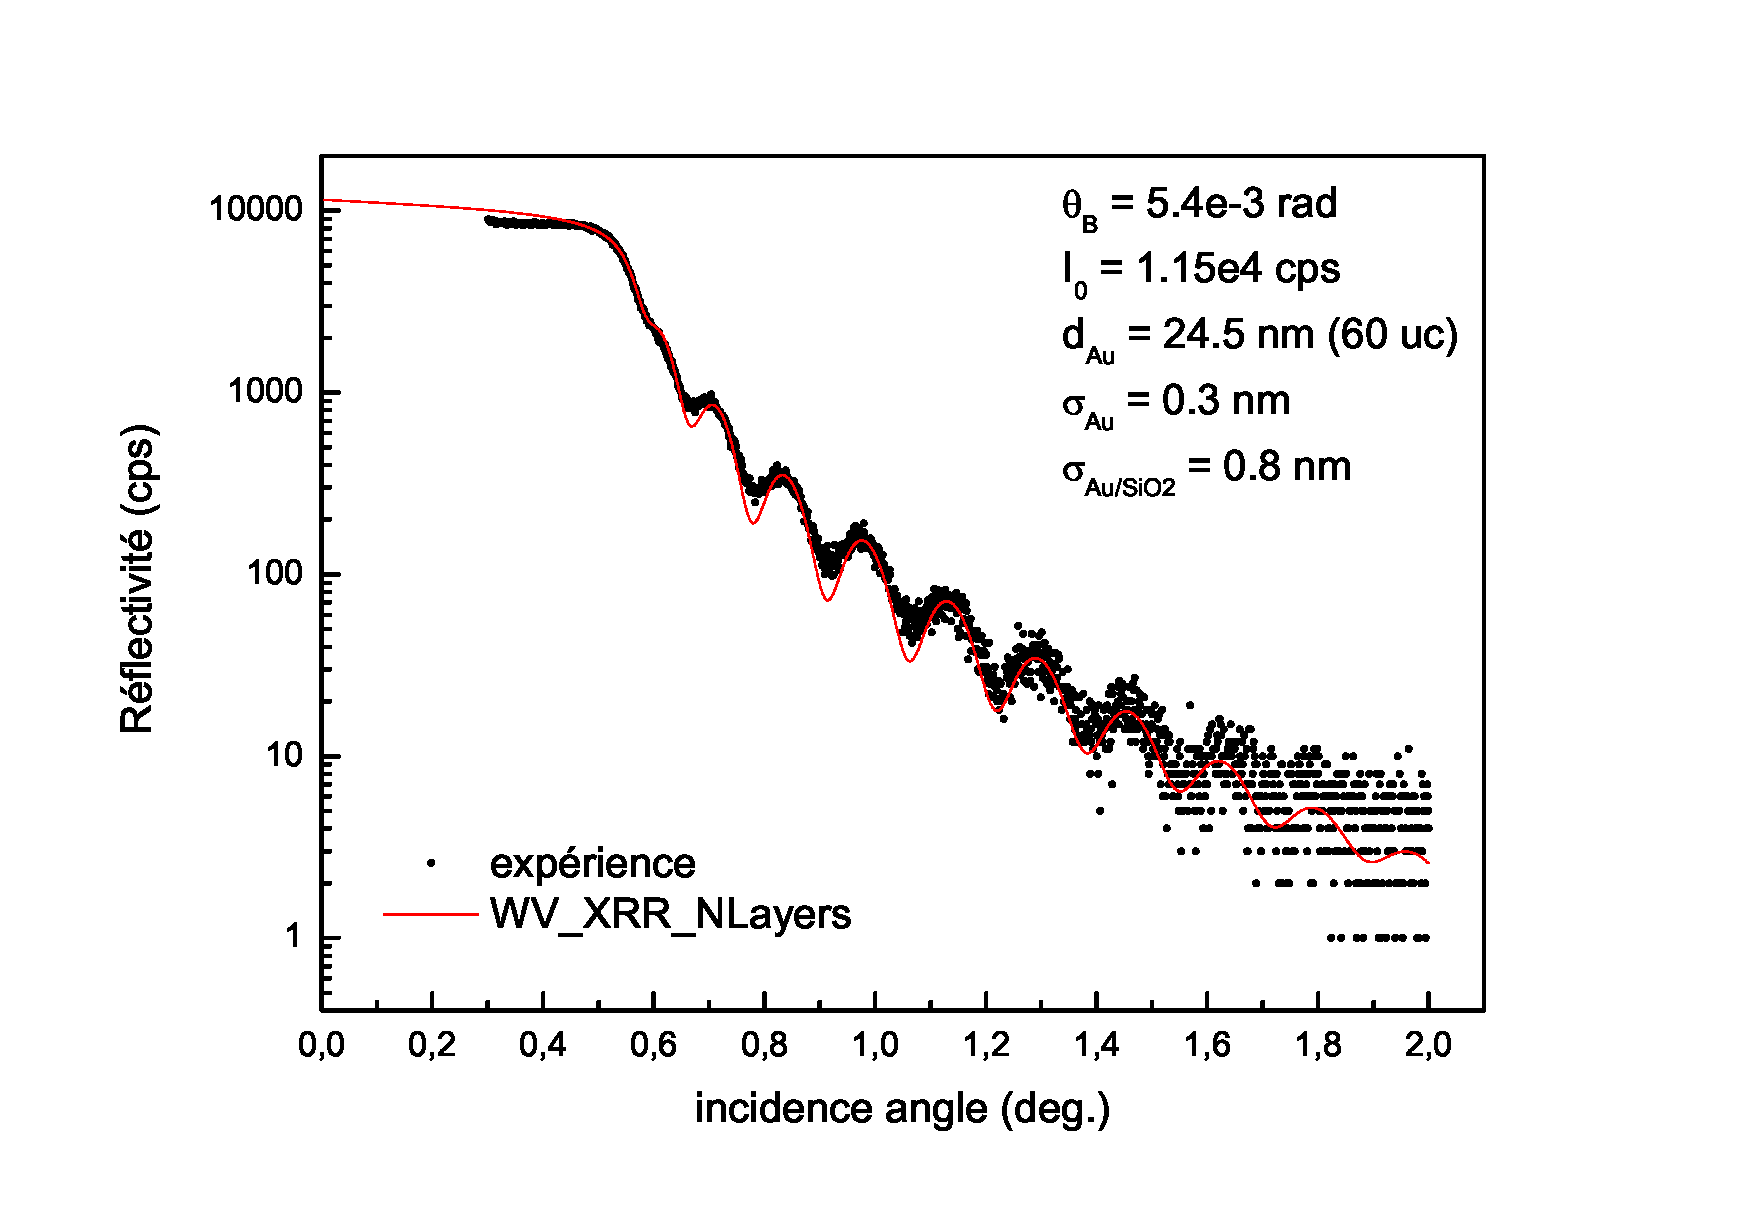
\includegraphics[width=0.5\textwidth]{./figures/GValidationAuQuartz.eps}
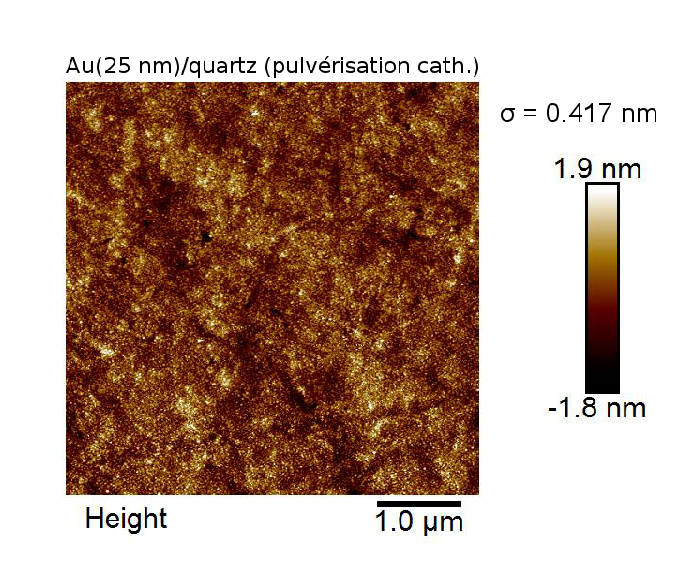
\includegraphics[width=0.5\textwidth]{./figures/AFM_Au.eps}


\iffalse
	\bigskip
	\textbf{\textsf{\'Etude de colles conductrices à base de nanoparticules d'argent}}

L'interconnexion constitue un facteur limitant majeur pour des applications au-delà de 200 $^\circ$C. Parmi les solutions existantes, comme les résines conductrices ou encore les alliages métalliques sans plomb chargés de nanoparticules conductrices, les pâtes à braser à base de nanoparticules d'argent présentent le meilleur potentiel de fonctionnement à très hautes températures, au-delà de 400 $^\circ$C. La réduction de la taille des grains à l'échelle nanométrique a permis de s'affranchir de l'application de pression durant le frittage, rendant cette technologie compatible avec un grand nombre de méthodes de fabrication.

Si les résidus des surfactants organiques évitant la solidification de l'assemblée de nanoparticules peuvent détériorer les performances globales de la brasure, le choix du dispersant offre une variété considérable de compositions possibles, ce qui rend les pâtes d'argent très versatiles. La modulation de la composition chimique permet ainsi d'ajuster des paramètres tels que la température de frittage, la distribution en taille des particules et les propriétés de mouillage en fonction de l'application. La performance globale d'une brasure est principalement déterminée par sa capacité à conserver ses propriétés au cours de son fonctionnement, et tout particulièrement au cours de cycles thermiques. La résistance d'une brasure à ce type de contraintes est intimement liée à la microstructure. Cette dernière résulte des transformations se produisant au cours du frittage et constitue une propriété centrale dans l'évaluation d'une brasure quelle que soit sa composition.

A été développée une méthode expérimentale d'analyse en temps réel de l'évolution de la microstructure d'une pâte à braser à base de nanoparticules d'argent durant le frittage. Cette méthode combine deux techniques de diffraction, électronique et de rayon X, pour sonder respectivement le début du frittage (petits volumes diffractants) et sa fin (matériau massif), de la thermogravimétrie ainsi que des mesures de résistance en temps réel. Ces techniques ont été appliquées à l'étude d'une pâte destinée à l'interconnexion de dispositifs tout-oxyde dans la perspective de fonctionnement au-delà de 400 $^\circ$C. La microstructure de la pâte calcinée se caractérise par des grains d'argent de l'ordre de 80 nm de diamètre. Le suivi en temps réel des transformations se produisant durant le frittage permet d'établir que cette microstructure est déterminée par un des surfactants introduit dans la solution colloïdale.
L'évolution de la microstructure en fonction de la température est illustrée dans la figure ci-dessous par les anneaux de diffraction (à gauche) et les diagrammes intégrés (à droite) à une température intermédiaire (en haut) et à la fin du frittage (en bas).
\par

\includegraphics[width=0.3\textwidth]{./figures/cadre_blanc.eps}
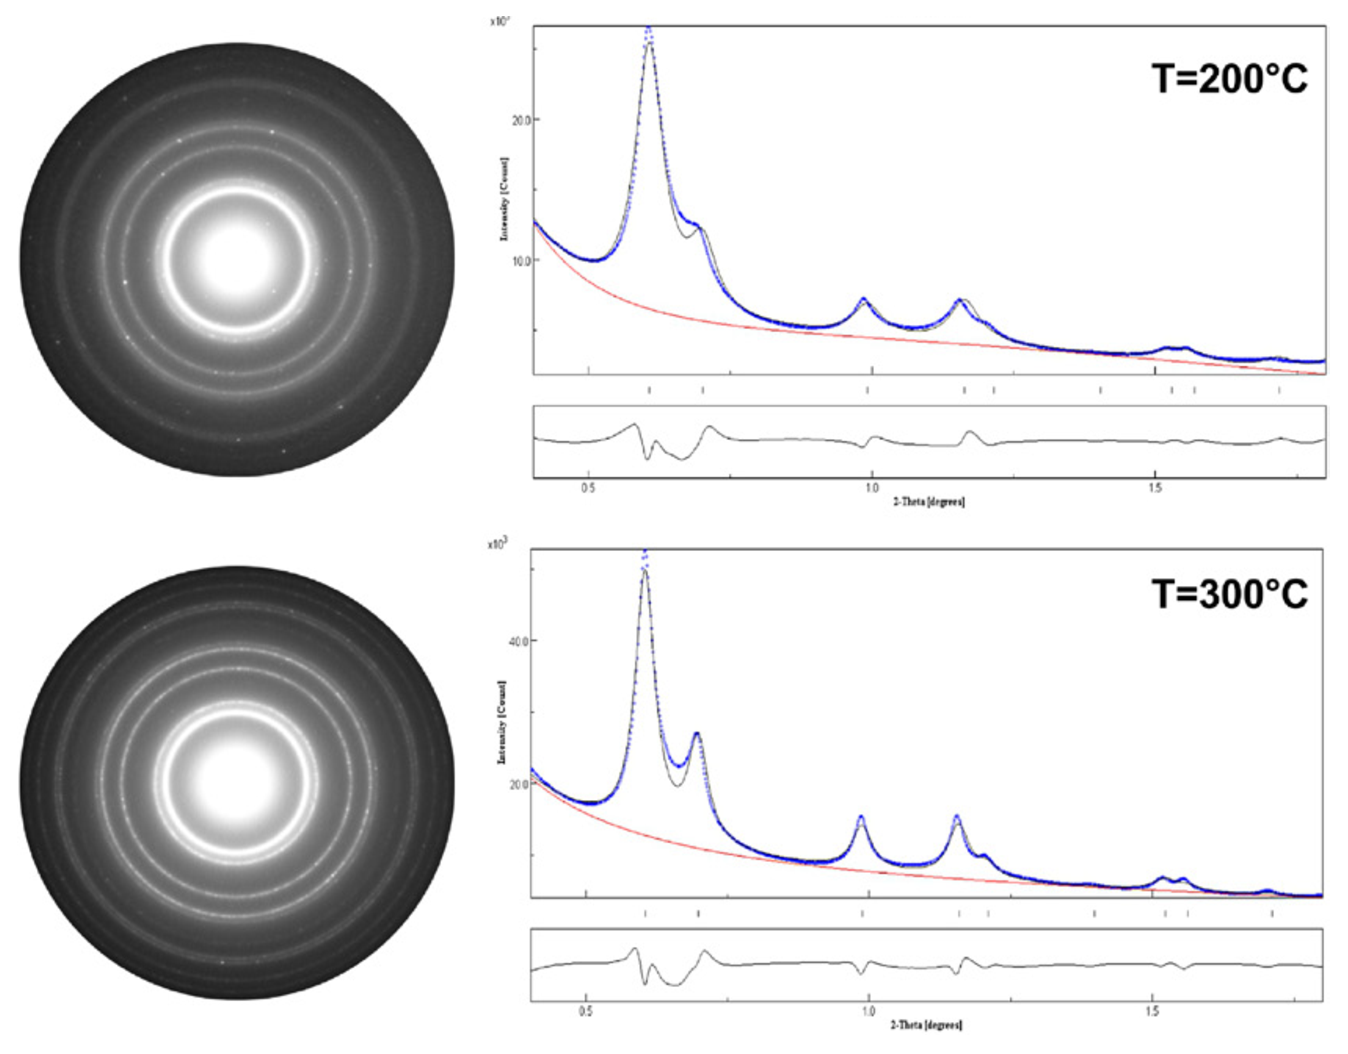
\includegraphics[width=0.4\textwidth]{./figures/ColCoNAg.eps}

\includegraphics[width=0.3\textwidth]{./figures/cadre_blanc.eps}


Pour ce projet, j'ai reçu le soutien d'un ingénieur d'étude, Mr Xavier Tassart, financé par le labex CHARM3AT en 2013-2014, en collaboration avec Dr. Eddy Dumas de l'Institut Lavoisier de Versailles.

Ces travaux sur les pâtes à braser à base de nanoparticules d'argent ont donné lieu à une communication orale au Symposium du Génie Electrique (Cachan, 2014) ainsi qu'à un article publié dans Journal of Physics D: Applied Physics en 2015.

Le projet s'est achevé par la réalisation d'une expérience de thermométrie par bruit thermique qui illustre une innovation possible permise par notre matériau: la mesure absolue de la température de surface d'un film résistif. Une partie de ce développement a fait l'objet d'un stage de M2. Cette expérience de principe valide la composition du matériau, son protocole de dépôt et sa capacité à lever le verrou que constitue le contact électrique jusqu'à 1000 K. 
\fi

\newpage
\input{projet_recherche.tex}

\newpage
\input{pratiques_pedagogiques.tex}
 
\newpage
%\cite{sene2017}
\cite{1804.07574}
\cite{scola2017}
\cite{Scola2015}
%\cite{wright2014}
\cite{Hamie2012115} %2012
\cite{ISI:000311968400074} % popova2012
%\cite{ISI:000308091500469} % wright2012
\cite{ISI:000301729200091} % berini jap 2012
\cite{ISI:000300459200039} % berini thin solid film 2012
\cite{PhysRevB.84.104429} %prb2011
\cite{JAP.110.043928} % jap2011
\cite{PhysRevB.81.174409}

\newpage


\nocite{*}
%\bibliographystyle{plain}
\bibliographystyle{unsrt}
%\bibliographystyle{publist}
\bibliography{biblio_perso_10}


\newpage
\section{Conférences}
\cventry
	{}
	{Oral}
	{Electric field driven metal-to-insulator transition at a Al/LaNiO$_3$ interface}
	{J. Scola, P. Nukala, B. Berini, Y. Dumont, B. Dkhil}
	{}
	{Réunion plénière, GDR MEETICC, janvier 2019, Dunkerque, France}
	
\cventry
	{}
	{Oral}
	{Oxide heterostructure with 10$^5$ \% electro-resistance}
	{J. Scola, B. Berini, Y. Dumont}
	{}
	{A.P.S. March meeting 2018, mars 2018, Los Angeles, États-Unis}
	
\cventry
	{}
	{Oral}
	{Brasure à base de nanoparticules d'argent : évolution en temps réel de la microstructure et
de la résistance}
	{Scola Joseph, Tassart Xavier, Dumas Eddy, Boullay Philippe, Jomard François, Vilar Christèle,
Veniaminova Yana, Gascoin Stéphanie}
	{}
	{Symposium de Génie Electrique EF-EPF-MGE 2014, juillet 2014, Cachan}

\cventry
	{}
	{Oral}
	{Interface induced coupling in films of YFeO$_3$}
	{J. Scola, W. Noun, E. Popova, N. Keller}
	{}
	{11th joint MMM-Intermag conference, Janvier 2010, Washington DC, Etats-Unis}

\cventry
	{}
	{Oral}
	{Dynamical study of the vortex lattice by transverse noise measurements}
	{J. Scola, A. Pautrat, C. Goupil, Ch. Simon}
	{}
	{ESF Vortex and PI-shift workshop, Mai 2004, Bad Münstereifel, Allemagne}

\cventry
	{}
	{Affiche}
	{Electric field driven metal-to-insulator transition at a Al/LaNiO$_3$ interface}
	{J. Scola, P. Nukala, B. Berini, Y. Dumont, B. Dkhil}
	{}
	{GDR OXYFUN, Octobre 2019, Caen, France}
	
\cventry
	{}
	{Affiche}
	{Oxygen vacancy creation and healing in ultra-thin films of LaNiO$_3$}
	{J. Scola, A. Senegas, B. Berini, Y. Dumont}
	{}
	{Workshop on Oxide Electronics, Octobre 2015, Paris, France}

\cventry
	{}
	{Affiche}
	{Resistivity and resistance noise in ultra-thin films of LaNiO$_3$}
	{J. Scola, A. Senegas, B. Berini, Y. Dumont}
	{}
	{CIMTEC, Juin 2014, Florence, Italie}
  
\cventry
	{}
	{Affiche}
	{Microstructure and electrical behavior of Ag-nanoparticles-based solderings}
	{Y. Veniaminova, J. Scola, E. Dumas, C. Mayer}
	{}
	{International Conference on Nanoscience + Technology, Juillet 2012, Paris}  
 
\cventry
	{}
	{Affiche}
	{Microstructure and self exchange coupling in a YFeO$_3$ film}
	{J. Scola, P. Boullay, W. Noun, E. Popova, A. Fouchet, Y. Dumont, N. Keller, I. Sheikin, P. Lejay}
	{}
	{SCTE avril juin 2012 Lisbonne, Portugal} 

\cventry
	{}
	{Affiche}
	{Microstructure and electrical behavior of Ag-nanoparticles-based solderings}
	{Y. Veniaminova, J. Scola, E. Dumas, C. Mayer}
	{}
	{SCTE 2012, Lisbonne, Portugal} 

\cventry
	{}
	{Affiche}
	{Artificial tuning of the critical current and the voltage noise by surface roughening}
	{J. Scola, A. Pautrat, C. Goupil, Ch. Simon}
	{}
	{Applied Superconductivity Conference, 2006, Seattle WA, U.S.A.}



\end{document}

\iffalse
\cite{PhysRevB.79.024507}
\cite{ISI:000254194400054}
\cite{ISI:000247468900049}
\cite{ISI:000248442200122}
\cite{ISI:000249049500060}
\cite{ISI:000240836700008}
\cite{PhysRevB.73.024508}
\cite{ISI:000242215600017}
\cite{ISI:000235042300007}
\cite{PhysRevB.72.012507}
\cite{PhysRevB.71.104507}
\cite{PhysRevB.71.064517}
\cite{ISI:000227645300005}
\cite{PhysRevB.69.224504}
\cite{brevetFermon}
\fi